\documentclass{template/openetcs_report}
% Use the option "nocc" if the document is not licensed under Creative Commons
%\documentclass[nocc]{template/openetcs_article}
\usepackage{lipsum,url}
\usepackage{supertabular}
\usepackage{multirow}
\usepackage{color, colortbl}
\definecolor{gray}{rgb}{0.8,0.8,0.8}
\usepackage[modulo]{lineno}
\graphicspath{{./template/}{.}{./images/}}

\begin{document}
\frontmatter
\project{openETCS}

%Please do not change anything above this line
%============================
% The document metadata is defined below

%Background color of boxes in process graphic
\definecolor{light-gray}{gray}{0.95}

%assign a report number here
\reportnum{OETCS/WP4/D4.3.3}

%define your workpackage here
\wp{Work-Package 4: ``Validation \& Verification Strategy''}

%set a title here
\title{openETCS Safety case for tool chain and processes}

%set a subtitle here
\subtitle{Process and Toolchain verification for the openETCS on-board unit software development}

%set the date of the report here
\date{December 2015} %\\ Revised April 2015}

%document approval
%define the name and affiliation of the people involved in the documents approbation here
\creatorname{Jan Welte]}
\creatoraffil{TU Braunschweig}

\techassessorname{Abdelnasir Mohamed}
\techassessoraffil{AEbt}

\qualityassessorname{Veronique Gontier}
\qualityassessoraffil{All4Tec}

\approvalname{Klaus-R\"udiger Hase}
\approvalaffil{DB Netz}

%define a list of authors and their affiliation here

\author{Jan Welte}
\affiliation{Technische Universität Braunschweig\\
  Institute for Traffic Safety and Automation Engineering\\
  Hermann-Blenk-Str. 42\\
  38108 Braunschweig, Germany\\
  eMail: openetcs@iva.ing.tu-bs.de \\
  WebSite: www.iva.ing.tu-bs.de}
  
\author{Raphaël Faudou}
\affiliation{Samares Engineering on behalf of ENSEEIHT}


\author{Francois Revest}
\affiliation{All4Tec}
%add yourself as author, if you contributed to the document



% define the coverart
\coverart[width=350pt]{openETCS_EUPL}

%define the type of report
\reporttype{Output Document}


\begin{abstract}
This document addresses the general quality and safety assurance concept implemented and applied by the openETCS development process and its supporting toolchain. Thereby, the it is shown how the overall openETCS development process principals presented in D2.3 and  additional document can be applied for a CENELEC confirm SIL 4 development, if the interfaces to the system development are complemented accordingly. For the generic safety argumentation it is shown hw the model design addresses the ETCS system hazards for the OBU Kernel.

\end{abstract}

%=============================
%Do not change the next three lines
\maketitle
\tableofcontents
\listoffiguresandtables
\newpage
%=============================

\chapter{Document Control}

\begin{tabular}{|p{4.4cm}|p{8.7cm}|}
\hline
\multicolumn{2}{|c|}{Document information} \\
\hline
Work Package &  WP4  \\
Deliverable ID & D 4.3.3\\
\hline
Document title & Process and Toolchain verification for the openETCS on-board unit software development \\
Document version & 1.0 \\
Document authors (org.)  & Jan Welte (TU-BS)\\
\hline
\end{tabular}

\begin{tabular}{|p{4.4cm}|p{8.7cm}|}
\hline
\multicolumn{2}{|c|}{Review information} \\
\hline
Last version reviewed & \\
\hline
Main reviewers (org.) & \\
\hline
\end{tabular}

\begin{tabular}{|p{2.2cm}|p{4cm}|p{4cm}|p{2cm}|}
\hline
\multicolumn{4}{|c|}{Approbation} \\
\hline
  &  Name & Role & Date   \\
\hline  
Written by    &  Jan Welte & WP4-T4.4 Task Leader  &  November 2015\\
\hline
Approved by & -- & -- & \\
\hline
\end{tabular}

\begin{tabular}{|p{2.2cm}|p{2cm}|p{3cm}|p{5cm}|}
\hline
\multicolumn{4}{|c|}{Document evolution} \\
\hline
Version &  Date & Author(s) & Justification  \\
\hline
0.1 & 18/10/2013 & Jan Welte &  Document creation \\
\hline  
%0.1 & 28/01/2014 & Jan Welte &  Extended Introduction  \\
\hline  
\end{tabular}
\newpage

% The actual document starts below this line
%=============================

\mainmatter

\chapter{Introduction}
\label{sec:introduction}

 The CENELEC standards EN 50126, EN 50128 and EN 50129 provide a basic life cycle process with specific artifacts which have to be produced during a system development. In this context presents the EN 50128 the specific life cycle and its artifacts for the software development. As this software operates in the system context it has to be defined in the system context which hazards have to be avoided or reduced to reach the required safety level. In this context safety is understood as protecting humans from harm resulting from the system as distinguished from security which covers protecting the system itself from hazards coming from the outside. To  do so the CENELEC standards can only provide guidelines how safety for a system shall be determined and assured by providing certain quality and safety management principles. These have to be adopted to the development methods applied during the system development. 
 
 As the openETCS project is related to a number of different system definitions like the overall railway system, the on-board unit, the kernel software and the development tool chain different safety aspects have to be taken in consideration. Only a small number of these can actually be determined in the openETCS context alone. Respectively, this document and all considerations concerning safety in openETCS are focusing on the principal functional safety of the openETCS on-board kernel software and it resulting principals which have to be applied if the software model and code shall be used in a specific context. To do so the specific development concept of openETCS is set in context to the CENELEC requirements and the underlying quality and safety management principals are shown to be integrated into the overall system management principal during further application of the openETCS results.


\section{Purpose}
\label{sec:purpose}

The hazard and risk analysis activities are part of the overall safety process which is defined in the EN 50129 as "the series of procedures that are followed to enable all safety requirements of a product to be identified and met". To ensure that the safety process is implemented and followed in a proper way during the development the EN 50129 requires a safety management. The management has to present and control all related activities and documentation over the life-cycle taking into account the approval mile-stones and review requirements. As the product life-cycle is an ongoing process and iterative changes are taking place, the management system has to ensure that the respective safety effects of every change is considered. The openETCS project does not cover the full development of an ETCS on-board unit, the tool and process verification in WP 4 and the resulting generic safety case are just providing confirmations how the openETCS toolchain and development process address safety relevant aspects at interface and in kernel design as well as requirements resulting for the use of openETCS kernel outputs. Hence, the purpose of this document is to provide an overview about the underlying quality and safety concepts established at the openETCS development.

As the movement characteristics of a train set specific limits in which a driver alone is able to avoid derailment or any kind of collisions, railway signaling and protection systems have been developed to ensure safe train movements. Respectively, the major parts of a train control system like ETCS includes functionalities which shall guarantee that the overall railway system does not get in a hazardous situation. Correspondingly, this document illustrates where identify hazards from the overall system analysis - if they are related to the openETCS software -  have been addressed in the development process and the kernel design. 

As the openETCS project does not produce an implemented train borne on-board system, the openETCS documents will not cover all specific software and hardware aspects which the EN 50129 requires for a sufficient safety case. Respectively, the openETCS results cannot be used without further work to demonstrate that a derived product using the openETCS kernel is compliant with all specified safety requirements. On this grounds WP 4 has arranged required information for the further use of the openETCS model as a generic safety case.

\section{Document Structure}
\label{sec:document-structure}

Although the openETCS software development process and the respective tool chain are closely connected, certain aspects should by address separately. The chapter \ref{toolchain} first presents the openETCS toolchain concepts and describes the tool classes categorization in the overall context. In addition the resulting qualification needs are addressed. Afterward, presents chapter \ref{sec:development-process} the development process of the openETCS and its artifacts. These are set in relation to the CENELEC lifecycle to address the needed interactions to adopted the openETCS kernel in a specific system development. As traceability is the core cross functionality for quality and safety management and central for reuse of software products and assessment, the final openETCS traceability concepts is presented additionally. The basic results how the existing ETCS system hazards have been addressed during the development is presented in chapter \ref{sec:safetycase}. Thereby, the four main safety case aspects system definition, quality management, safety management and functional safety are addresses separately.

\section{Document Evolution}

This document is based on the results of the various iterations during the WP 4 work and shall present the overall concept for the openETCS development. As the openETCS ETCS OBU reference model is an ongoing development, this document can not provide a final status which can be used as a assessable safety case for the direct implementation. However this document presents the concept and principals applied in openETCS which can be used and extended to integrate the OBU reference model in specific applications.

The openETCS development plan presented in chapter \ref{sec:development-process} is based on the current version of the Quality Assurance Plan, the D2.3 deliverables group discribing the development process and WP 7 outputs concerning the toolchain. Concrete methods to verify and validate safety relevant properties derived from the hazard control methods described in this document, are presented in depth   in the Verification and Validation plan and the specific results are documented in are respective verification and validation reports.

\section{Reference Documents}
\label{sec:refdoc}

This document essentially refers to the following standards, ETCS specification documents and openETCS project documents.

\begin{itemize}
\item \textbf{ISO~9000} --- 12/2005 --- \emph{Quality management}
\item \textbf{ISO~9001} --- 12/2008 --- \emph{Quality management systems — Requirements}
\item \textbf{ISO~25010} --- 03/2011 --- \emph{Systems and software engineering -- Systems and software Quality Requirements and Evaluation (SQuaRE) -- System and software quality models}
\item \textbf{CENELEC EN~50126-1} --- 01/2000 --- \emph{Railways applications –- The specification and 
demonstration of Reliability, Availability, Maintenability and Safety (RAMS) –- Part 1: 
Basic requirements and generic process}
\item \textbf{CENELEC EN~50128} --- 10/2011 --- \emph{Railway applications -- Communication, signalling and 
processing systems -- Software for railway control and protection systems}
\item \textbf{CENELEC EN~50129} --- 05/2003 --- \emph{Railway applications –- Communication, signalling and 
processing systems –- Safety related electronic systems for signalling}
\item \textbf{CCS~TSI} --- \emph{ CCS TSI for HS and CR transeuropean rail has been adopted by a Commission Decision 2012/88/EU on the 25th January 2012}
\item \textbf{SUBSET-026} 3.3.0 --- \emph{System Requirement Specification}
\item \textbf{SUBSET-091} 3.2.0 --- \emph{Safety Requirements for the Technical Interoperability
of ETCS in Levels 1 \& 2}
\item \textbf{SUBSET-088} 2.3.0 --- \emph{ETCS Application Levels 1 \& 2 - Safety Analysis}
\item \textbf{OpenETCS FPP} --- \emph{Project Outline Full Project Proposal Annex OpenETCS} -- v2.2
\item \textbf{OpenETCS D2.2} -- Report on CENELEC standard
\item \textbf{OpenETCS D2.3} -- Definition of the overall process for the formal description of ETCS and the rail system it works in 
\item \textbf{OpenETCS D2.4} -- Definition of the methods used to perform the formal description
\end{itemize}


%%%%%%%%%%%%%%%%%%%%%%%%%%%%%%%%%%%%%%%%%%%%%%%%%%%%%%%%%%%%%%%

\section{Glossary}
\label{sec:glossary}



\begin{tabular}{rl}
%\textbf{ACedit} & Assurance Case Editor \\ 
%\textbf{ARM} & Argumentation  Metamodel \\ 
\textbf{ESF} & Eclipse Safety Framework \\ 
\textbf{ETCS} & European Train Control System \\ 
\textbf{ERA} & European Railway Agency \\ 
%\textbf{FMEA} & Failure Mode Effect Analysis \\ 
%\textbf{GSN} & Goal Structured Notation \\ 
%\textbf{MoRC} & Management of Radio Communication \\ 
%\textbf{RAMS} & Reliability, Availability, Maintainability and Safety \\
\textbf{SIL} & Safety Integrity Level \\ 
\textbf{SRS} & System Requirement Specification \\ 
%\textbf{THR} & Tolerable Hazard Rate \\ 
\textbf{V\&V} & Verification \& Validation \\ 
\end{tabular} 




%\section{Background Information}
%\label{sec:Background}


\chapter{Tool Chain}
\label{toolchain}
\section{Overview}

As it has been state in the openETCS FPP one of the goals  is to "Provide a tool chain and process/methodologies for developing an on-board software that can fulfill the CENELEC requirements for SIL4 software" [FPP]. To do so O~7.3.2 Tool chain Design Specification state that the tool chain  provides tool support for a formalized specification of SRS and an executable code of the OBU. In addition cross cutting tools for traceability, version management, integration and documentation as well as specific V\&V activities are needed.

Overall O~7.3.2 distinguishes two kind of tools:
\begin{itemize}
\item Development tools: those used along the phases of the software development process including V\&V  (Requirement engineering, modeling ...).
\item Management tools: those used transversely during the complete development process (version
management, requirements traceability ...).
\end{itemize}

In doing so the development tools are mostly split in design and in V\&V tools as these are used by the two different sides od the development. Do to the separation of responsibilities as it is required by the CENELEC process (see D2.3 for details concerning openETCS) these tools are mainly used by different groups. The management tools are also refereed to as Cross-Cutting Tools as their functionality is used during different development phases and activities.

\begin{figure}[h]
\centering
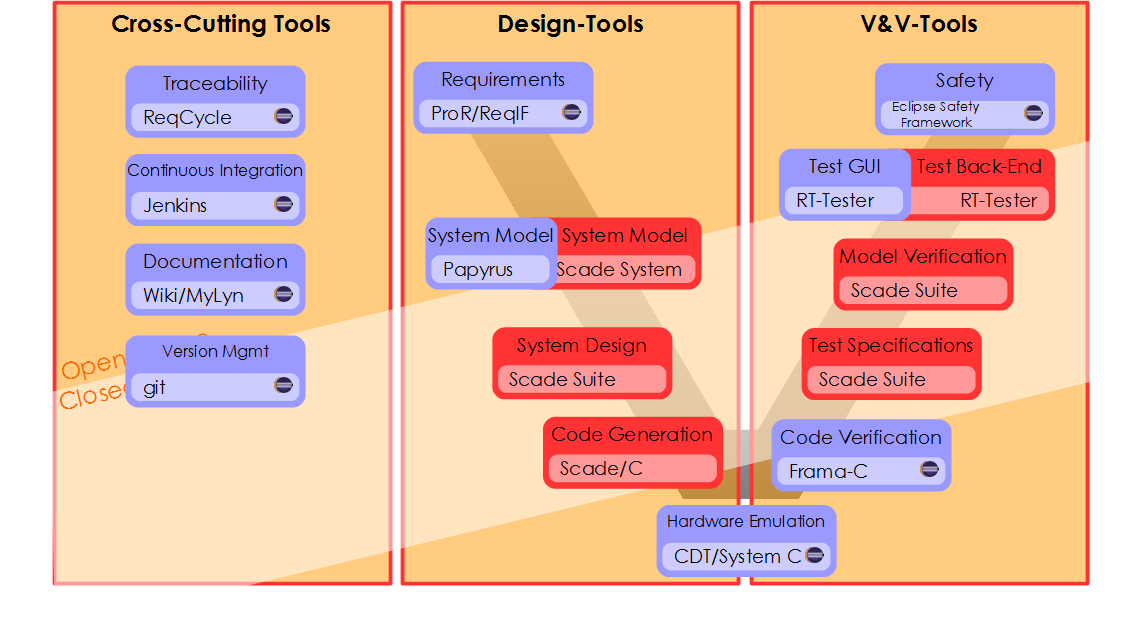
\includegraphics[width=0.9\linewidth]{./images/Toolchain-New-Version-V-Model-Nov-2015}
\caption{Core openETCS Toolchain}
\label{fig:Toolchain-New}
\end{figure}

The main components of the openETCS toolchain and there allocation to the V-Model development are presented in figure \ref{fig:Toolchain-New}.  The current version of the openETCS toolchain essentially uses two tool platforms, the open source platform based on Eclipse and the close source platform of SCADE. The interfaces been both platforms are SysML on the Architecture level and C Code on the Source Code level. Additional tools mainly V\&V related are using on of these artifacts formats as input. 

Although the main functionality and artifact exchanges have been sampled during the openETCS development, it has not been possible for the development to continuously use the completely integrated toolchain as shown in figure \ref{fig:Toolchain-New}. Due to recurring challenges with Papyrus and SCADE SysML models the WP 3 design team has mainly worked with the SCADE platform, to ensure an usable product. Thereby, it has been difficult to establish traceability between the open source and the SCADE parts and to push tool qualification.

\section{Tool Qualification}

The CENELEC EN 50128 standard defines the required tool qualification as measures to ensure that a failures of the tool cannot directly be taken into the tool-set output. Thereby, failures have to be addressed in relation to the overall safety. Accordingly, tools are categorized in three classes.

\begin{itemize}
\item Tool class T1: No generated output can be used directly or indirectly to the
  safety critical executable code;
\item Tool class T2: Verification tools, e.g. that can not introduce
  errors to the safety critical executable code but those tools may fail to detect errors or
  defects;
\item Tool class T3: Generated output directly or indirectly  as part of the
  safety critical executable code.
\end{itemize}

Depending on it's use in the overall development toolchain a tool needs to satisfy the respective tool class. D2.2 gives an overview about the general requirements for the tools needed by the different tool classes. O~7.3.2 shows various methods how tools can be qualified in these classes. Thereby, not only a tool can be qualified for each other, but also the toolchain integration in a tool platform has to be checked for potential failure. This includes mechanism such as exchange formats, artifacts versioning, time-stamping operations. As the openETCS toolchain is mainly based on two tool platforms it uses the main principals already ensured at these platforms. 

Nevertheless a complete definition of interactions between these tools is needed to fully qualify the openETCS toolchain as it is. The main tools contained in the openETCS development toolchain based on D7.3 and D2.3 are listed in table~\ref{tab:ToolCat} and categorized according to the tool class needed for the intended use. The justification gives the current state of qualification. Nevertheless, these list can only be seen as the initial point, as an in-depth definition and failure analysis of the actually used tool chain would be needed for a real development process. As openETCS was a research project the focus was to establish the functionality which then can provide the basis for a qualification. However, the use of the close source platform SCADE was primarily driven by its already existing qualification, which has not been available at open source level.

\begin{center}
\tablecaption{OpenETCS toolchain and categorisation}
\label{tab:ToolCat}
\tablehead{\hline Tool & Support Activity & Tool Class & Justification \\ }
\tabletail{ \hline \multicolumn{4}{|r|}{Continues on next page} \\ \hline}
\tablelasttail{\hline}

\begin{supertabular}[H]{|p{2cm}|p{4cm}|p{2cm}|p{5cm}|}
\hline ProR & Requirements management & T1 & \\
\hline Papyrus Editor & Definition of the model architecture & T1 & \\
\hline Papyrus SysML checker & Check SysML conformity of the model & T2 & \\
\hline SCADE System Editor & Import and additional definition of model architecture & T1& \\
\hline SCADE Editor & Low-level modeling and code generation & T1 & \\
\hline SCADE Code Generator & Code generation & T3 & \\
\hline Bitwalker & Generation of data structures for modelling & T3 & \\
\hline Frama-C & Code analysis & T2 & \\ 
\hline RT Tester & Model-based testing & T2 & \\ 
\hline Eclipse Safety Framework & Safety assessment of error propagation& T2 & \\
\hline ReqCycle & Traceability & T1 & \\
\hline Jenkins & Tool integration & T3 & \\
\hline Wiki/MyLyn & Documentation & T1 & \\
\hline Git & Versioning \& Traceability & T3 & \\
\end{supertabular} 
\end{center}

As the WP 3 and WP 7 activities have mainly been focused on establishing tool chain functionality, it has not been possible to provided openETCS specific qualifications for all T2 and T3 tools. But as SCADE Suite and the respective KCG for automatic C Code generation already provide a certification in respect to EN 50128 SIL 3/4, the basis for the overall toolchain qualification already exists. Anyhow for a concrete development use the specifically the Cross-Cutting tools and the V\&V tools have to be analyzed further to ensure complete failure detection.

\section{SCADE}

SCADE is at once  a formal modeling language and tool suite for the development of safety-critical embedded systems. SCADE has been used for more than 15 years to develop a broad range of control applications in the avionics, rail, and automotive domains. The SCADE platform containing among others SCADE System Editor, SCADE Editor, SCADE Display and their respective KCGs builds the main productive part of the openETCS toolchain. The main design work by WP 3 has been done with the SCADE Editor and all automatic generated code used has been created based on the SCADE Editor and SCADE Display models. As the SCADE language used as means of description is  an executable language with a deterministic semantics, the automatic code generation has been certified for C and Ada Code. Therefore, the use of SCADE as core of the productive design toolchain satisfies the tool requirements. The automatic checks done during the code generation also check consistence of the initial model.

The certification only concerns the actual Code generation based on the SCADE Model. To ensure QA in the design process and to qualify the overall toolchain modeling guidelines and quality measures for version and configuration management are needed. During the openETCS development it had to be ensured that github does not merge different versions of a xscade SCADE model file as this caused consistence problems. The xml format used by SCADE is not compatible with the github merging principals. Therefore, the openETCS project used separated model parts and check out principals to ensure that only one personal at a time is allowed to change a file. Nevertheless, a complete document by WP 3 and WP 7 listing all established measures and coding rules to ensure model consistency has not been provided at this point. This does not directly creates any safety related failures as SCADE clearly identifies consistence problems and the git configuration management provides options to retrieve the stable versions.


\section{Eclipse Safety Framework}

ESF is a framework for model based safety analysis. The model of the system or software to analyze must be described in a format compliant with the tool Papyrus. The leaf components of the hierarchical description of the system are called “blocks”. Once the model has been imported, a local dysfunctional analysis is made. The local dysfunctional analysis consists in establishing different Boolean equation for every block (logical links between the failure modes of the block, the failure modes of its inputs and the failure modes of the output of the block). This analysis is local because only the dysfunctional behavior of the block is analyzed. Once all blocks have been analyzed, the feared events are defined on the associated port. The propagation algorithm computes the fault tree from the feared events and shows which block failure modes contribute to which feared event.

For OpenETCS, the SysML model of the ETCS OBU has been imported in ESF. The structure of the model, links and components, are then recognized by ESF. Some problems in the SysML model have been detected during the ESF importation: links deleted in the graphical view and not in the textual view, connector link without destination port or target port.

The model behavior is described in the document D3.5.3 that was our basis for performing the dysfunctional analysis. For proof of the concept, only one feared event has been defined and analyzed: erroneous error message in the posRepHeader to the train. Once the local analysis has been done, a propagation of failure modes has been performed and the fault tree has been automatically computed. 
The analysis of the fault tree has shown that all the components were critical because any error on the equipment affects the output of the system. The SIL4 classification of this equipment is thus correct and cannot be reduced. It could be interesting to make the system safer by performing a checksum on the error message all along the process. Another proposal is to verify whether all input are consistent with the system specification.

\section{Summary}
\label{summary-tool}

Overall the verification of the toolchain has the result that the openETCS toolchain itself is consistent and provides the basic required functionality for the development. In particular the design tools starting at the requirement level with ProR and going via Papyrus to SCADE Suite are stable and mostly already coordinated concerning the artifact interfaces. Specifically the SCADE part is already well proven in use and also provides the needed qualification documents for a SIL 4 development. 

For nearly all other tools a proper qualification according to the tool class used in the development toolchain could be reached but has not been address up to now. Especially, the Cross-Cutting tools have to be checked in an in-depth  analysis to qualify them against potential failures. Any adopter of the openETCS toolchain has to do an analysis based on the specific configurations of artifacts and tools he is using for his development.


\chapter{OpenETCS Development}
\label{sec:development-process}

The main goal of the openETCS project is to develop a model of the ETCS OBU kernel in a CENELEC conform but agil development process. As presented in-depth in D2.3 and its additional deliverables the openETCS Software development process follows the basic EN~50128 lifecycle but has adjusted its artifacts and development phases to accommodate the model-based development based on the openETCS toolchain and the agile development principals. 

The current ETCS OBU SCADE model and the corresponding generated C Code is the resulting product of this development as the demonstrator parts of the project are examples for the multi platform use of the software and only serve as validation tools or the software functionality.

\section{overview}

As presented in-depth in D2.3 and its additional deliverables the openETCS Software development process follows the basic EN~50128 lifecycle but has adjusted its artifacts and development phases to accommodate the model-based development based on the openETCS toolchain and the agile development principals. The resulting openETCS development lifecycle is derived in D2.3a and shown in figure \ref{fig:lifecycle2}.

\begin{figure}[hbt]
  \centering
  \def\svgwidth{.9\textwidth}
  {\tiny
  \input{./images/Prcss2_3a-03.pdf_tex}}
  \caption{openETCS Development Lifecycle}
  \label{fig:lifecycle2}
\end{figure}

\section{Compatibility to CENELEC standards}

In contrast to the EN~50128 lifecycle, the openETCS lifecycle is not a full system development as hardware is not part of openETCS. The development only aims at the OBU kernel which is part of the  ETCS EVC and the overall ETCS system. Therefore, the substantial superordinated system information have to be considered during the openETCS system design. This is represented in this D2.3a lifecycle.

Furthermore, the openETCS lifecycle includes the software component design in the software architecture and design phase, as this those activities get closely connected in the agile model-based development. The SCADE models with there modular architecture development allow a dynamic design process which combines top-down elements for the system architecture to the single component by refinement as well as bottom-up work from basic components which are integrated step by step in the architecture. Both approaches have been used for different parts of the SRS during the openETCS project. As the high level SCADE integration models and the simulation test ensure consistency between all integrated modules this single phase represents the various agile iterations.

As correctly state in D2.3a all EN~50128 phase after validation are not part of the openETCS project and therefore not detailed at the moment. Nevertheless, the openETCS foundation and all adopters have to define a clear maintenance process after the end of the openETCS project. 

\section{Process Implementation}
\label{sec:proc-impl}

Since the openETCS development process shown in the previous section as just emerged over the duration of the project, the implementation of the process has also been a continuous process. Due to many challenges with supporting tools and coordination between process partners has the work main been concentrated on the actual design and implementation work. This has been performed in several agile iterations and in accordance with open ETCS release principles as presented in D2.3b. Functionality and integration test have been performed on parts of the system by WP~4 as these have been available in the releases.

Due to the focus on implementing and providing a final openETCS OBU Kernel model and supporting demonstrators the work has been driven by directly designing from the SRS. Accordingly, it has to be stated in this verification report that the actual sub-system specification for the openETCS OBU Kernel and the specific software specification as stated figure \ref{fig:lifecycle2} phase 1 and phase 3 have been very limited. In combination with the raw size of the openETCS model this aspect made it difficult to explicitly allocate specific model functions to the high level SRS requirements. This clear requirements refinement to software level is laking in the implemented openETCS process and has to be supplemented if the openETCS model should be used in a SIL 4 development context. However, the modular model structure and the existing architecture verification provide the basic information to complete the process implementation in a sequential use.

\section{Traceability}

Requirement traceability activity consists in ensuring that all product engineering artifacts (including verification means) can be traced to an originating stakeholder requirement either directly (direct link) or through other requirements derived from stakeholder requirements. It means creating links but also manage their status (created, confirmed...) and potentially their deletion.

Concerning OpenETCS, there are several needs for traceability but main ones concern definition of links between SRS-Subset 26 requirements and two models:
\begin{itemize}
\item OpenETCS architecture SysML model (System, subsystem, SW functions), edited with SCADE System tool
\item OpenETCS OBU formal executable software model (SW architecture, SW functions, detailed design), edited with SCADE Suite tool
\end{itemize}

Figure \ref{fig:openETCSTraceabilityMainPriority} illustrates all required traceability links needed to achieve current design verification and highlights main priority (arrows with largest size).

\begin{figure}[htbp]
\centering
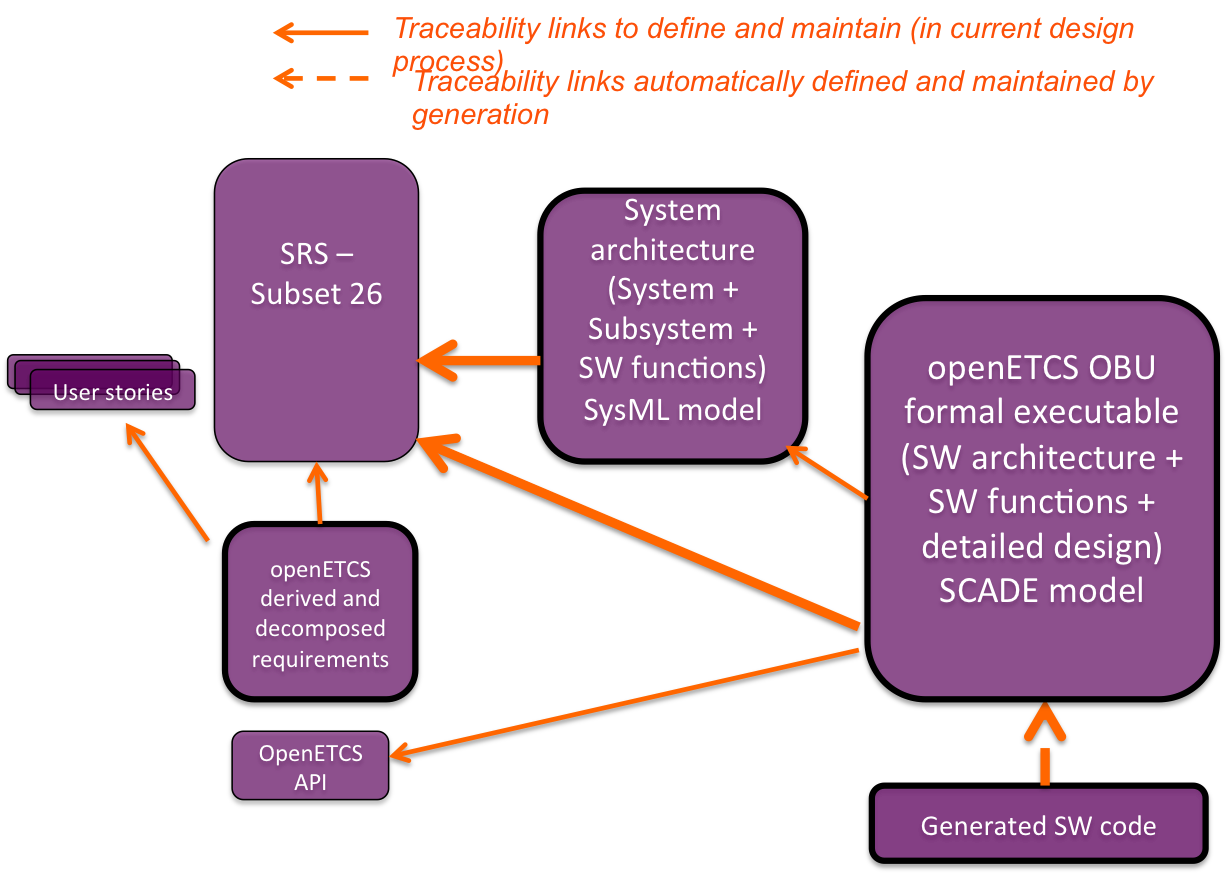
\includegraphics[width=.9\linewidth]
{./images/openETCSTraceabilityMainPriority.png}
\caption{\label{fig:openETCSTraceabilityMainPriority}OpenETCS traceability chains for current design with highlight on main priorities}
\end{figure}

OpenETCS tool chain currently supports ability to create links between:
\begin{itemize}
\item SRS Subset 026 .ReqIF requirements and additional requirements => through ProR integrated tool,
\item SysML architecture model and SRS Subset 026 .ReqIF requirements through ReqCycle integrated tool
\end{itemize}
 
\textbf{Note:} it is also possible to create links between SCADE Model and SRS Subset 026 .ReqIF requirements through SCADE Suite RM Gateway and ReqTify traceability product but it is not an open solution and it requires additional licenses. Therefore that approach was used only by a few partners and was not considered as conclusive. There are pending investigations to provide alternate open solutions to support edition of those traceability links.

Similarly to the overall development process traceability as the central crosscutting function and the corresponding tool support have just been established over the project duration. Due to missing tool support and licenses for different project partners trace between SRS requirements and SCADE models have not been set consistently. All overall architecture parts are linked a range of ETCS specifications, but the potential detailed linking of different basic functional blocks in SCADE, which eases the understanding of the model for V\&V and further use has not been established. Nevertheless, the main functions are commented in detail and these comments refer to specific parts of the SRS. Though the versatile use of automated traceability links between requirement, model and test abstractions, which could be provided by the openETCS development process and toolchain, was not been exercised.   


\section{Summary}
\label{summary-process}

Overall the verification of the openETCS process has shown that the general process used in openETCS is based on the EN~50128 lifecycle and also it uses agile development principal provides all required artifacts. The combination of architecture and design and component design phases is due to the used model-based development which combines top-down and bottom-up development. As the consistency for interfaces and functionality allocation is ensured during the regular model integration this process verifies the EN~50128 QA requirements. Also the available methodology and tool support for traceability allows to maintain the connections between iteratively developed requirements, specifications, models and tests as well as all supporting documentation.

However the actual implementation in the openETCS project has been found to lack activities concerning  the sub-system and software specifications documentation. Do to the focus on building a model the design team has derived their software specification base on the SRS and has directly implemented them in executable SCADE models for functional verification. This makes it difficult to follow and verify intermediated analysis and architecture processes between the ETCS system SRS and the actual OBU Kernel model. Especially as the tool challenges have limited a consistent establishment of traces between SRS, SysML architecture and Scade specification models. This has also limited the independent testing by WP 4 to mainly architecture verifcation and functional validation, as to extract concrete requirements for a software verification have been laborious. 

Overall the various exemplary applications for all phases of the development lifecycle have shown that the openETCS development process and the supporting toolchain are suitable in the described way. 


\chapter{Generic OpenETCS Safety Case}
\label{sec:safetycase}

The purpose of a safety case is to coherently present all available evidence to the assessing authority that the development has been done according to the required standards and that it has taken a needed safety properties into account. As the openETCS project just provides a n ETCS OBU kernel model without any specific target hardware it is not an independent assessable part. So this chapter provides the basic measures and safety allocations which have to be addressed by any adopter using the openETCS OBU Kernel software. Thereby, it is distinguished between basic assumptions, safety argumentation and evidences for the openETCS development as far as this already exist. To do so the chapter addresses the four main parts of a safety case according to the EN~50129 in the following sections:

\section{System/ Sub-System Definition}

\begin{figure}[htbp]
\centering
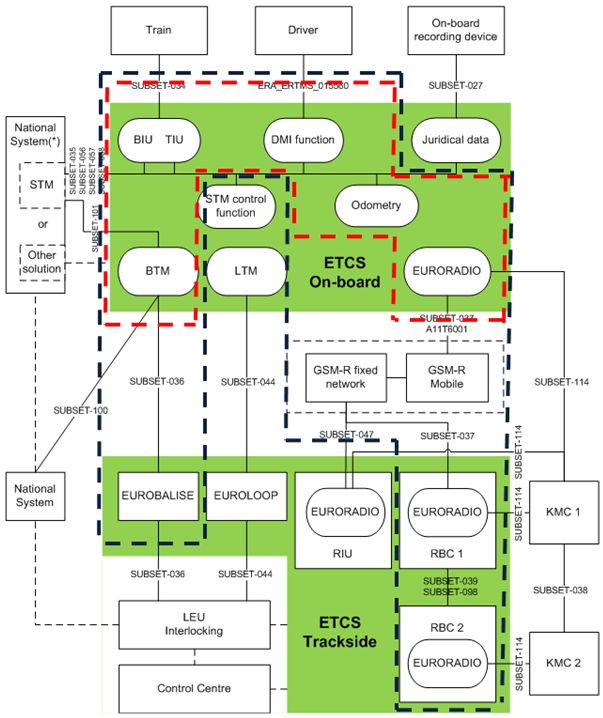
\includegraphics[width=.75\textwidth]{images/ArchitectureSRS}
\caption[]{Scope of openETCS OBU model system according to ERA TSI Chapter 2.5.}
\label{f:architecture_srs}
\end{figure}

As already stated above the openETCS development addresses the ETCS OBU Kernel, which runs on the EVC. 
As presented in the final architecture document D3.5.4 this does not include all ETCS components on-board as openETCS has the project decided to to time and effort limitations to not implement the LTM, JRU and STM components of the ETCS system structure defined in ERA SRS. The detailed systema and sub-system limits in ETCS are shown in figure \ref{f:architecture_srs}. In addition to the primary scope of openETCS OBU model, which are marked by the dashed red line, also certain parts of the ETCS trackside (e.g.~Eurobalise and RBC blocks) have been addresses for testing and validation purposes. These have been also been modeled in SCADE to allow the agile simulation and testing processes.  The scope of this integrated test environment is shown by the dashed black line in figure~\ref{f:architecture_srs}. A SysML representation of the overall ETCS architecture and the interfaces is shown in figure~\label{f:top_level}. The external interfaces are used for the communication between the openETCS OBU and systems out of the scope of the openETCS project and the ETCS Onboard Unit System. All interfaces as presented in detail in D3.5.4 as well as in their respective SysML and SCADE model specifications. 

\begin{figure} [htbp]
\centering
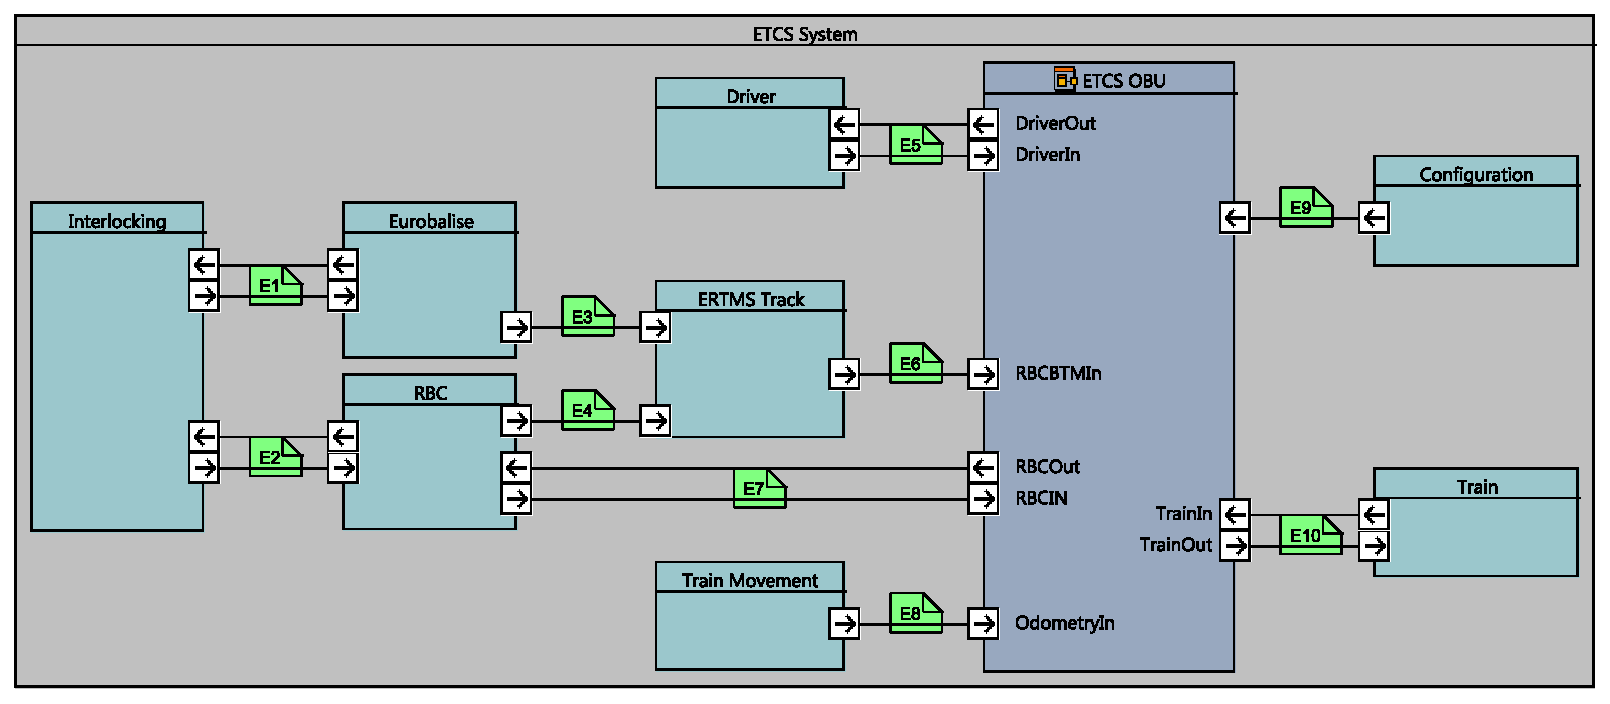
\includegraphics[width=0.9\textwidth]{ETCS_system.pdf}
\caption{ETCS architecture with external interfaces}
\label{f:top_level}
\end{figure}

Nevertheless, the extended scope is not part of the sub-system OBU kernel software and respectively not part of the developed product itself. Figure~\ref{f:ETCS_OBU_decomposition} shows the limits of the OBU Kernel and its internal interfaces, as they are implemented during the development process.

\begin{figure} [htbp]
\centering
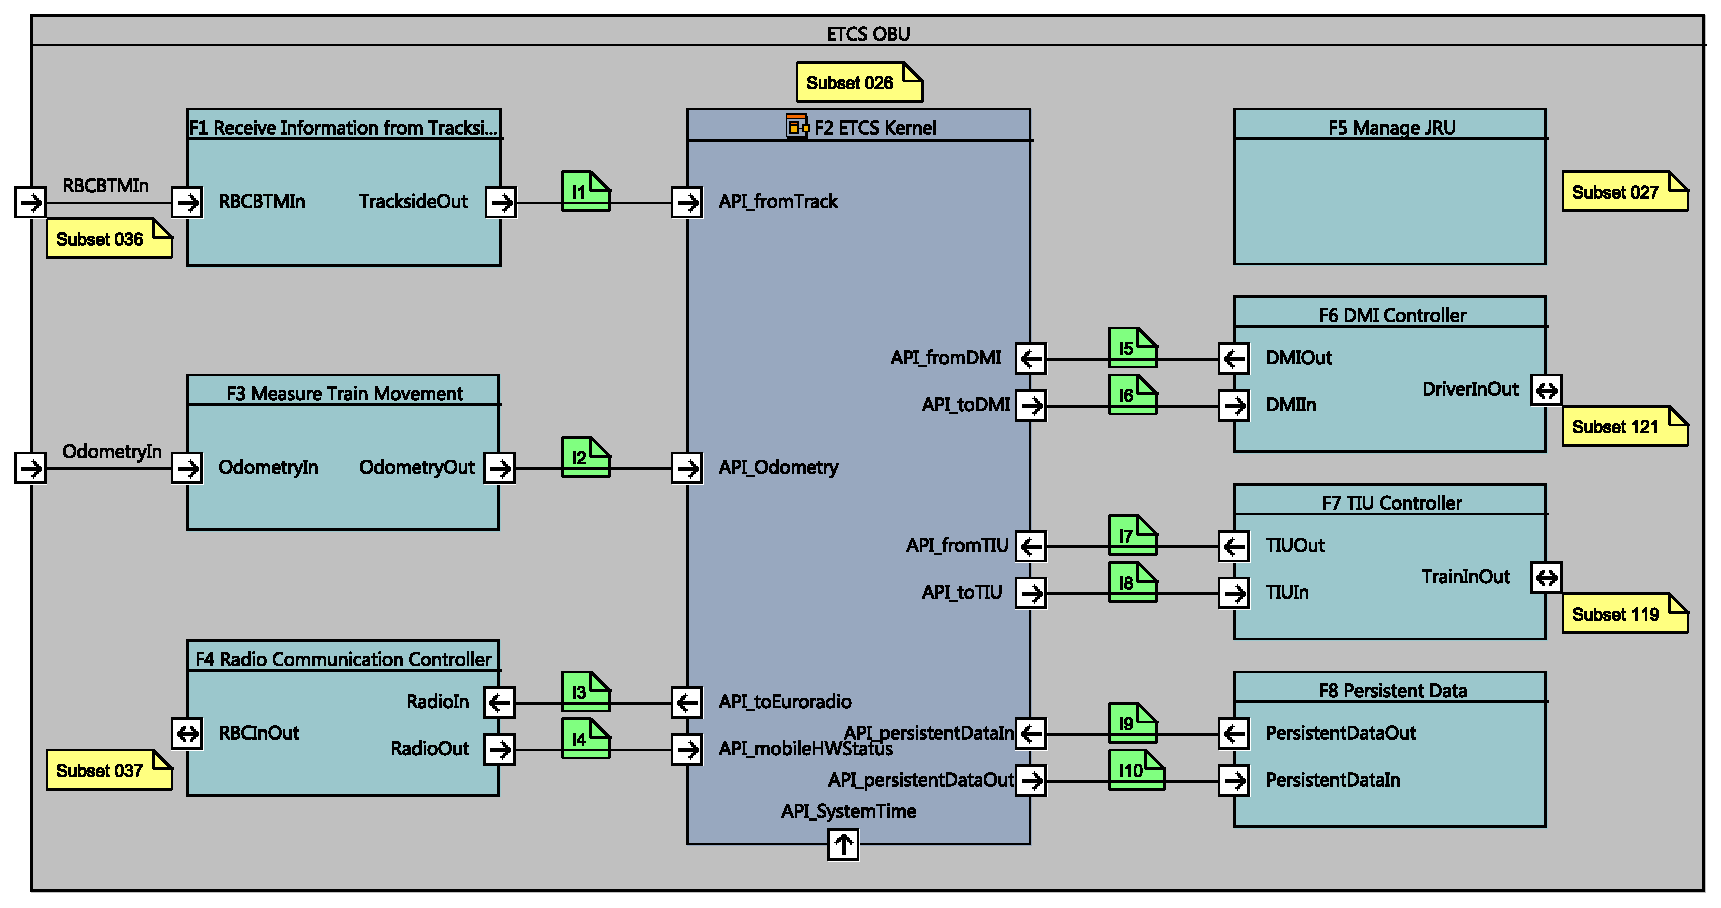
\includegraphics[width=0.9\textwidth]{images/F2_ETCS_Kernel.pdf}
\caption{ETCS OBU system architecture view with internal interfaces}
\label{f:ETCS_OBU_decomposition}
\end{figure}

A detailed definition for the sub-system and the integrated test environment is given in D3.5.4 and all associate outputs. Basis for all system definitions is the standardized ETCS architecture in the SRS and all corresponding ERA documents. The only actual product of the openETCS development process is the OBU Kernel software with all  primary

\section{Quality Management}

The main QA principals used in openETCS are defined by D1.3.1 the QA-Plan. The main principal applied over the whole openETCS process are the open continuous review process and the github based configuration management. I this way it is ensured that only commiter as qualified persons can directly provide content. Other contributions are only accepted as pull request if a commiter checked the content. In this way the as contributions are signed by the github account an could be redone if unwanted effects are found during following tests.

\section{Safety Management}

As in detail presented in D4.2.3 the safety case for a system has to demonstrate that during the development process the higher-level safety requirements have been addressed and that accordingly the on-board software satisfies the safety level. This requires traces from high-level hazardous events to all subsystem requirements allocated to the software architecture and their verification and validation. 
As the openETCS design has only focused on the functional implementation of SRS requirements, degraded modes have not been addresses consistently. Only cases specifically state in the SRS have been implemented.

However, the design and architecture specification presented in D3.5.4 for the OBU Kernel software and it components state constrains taken into account fo each interface. For example the track message interface providing BTM and Radio messages expects to receive only one message every cycle, hence this assumption is carried through the whole input management functionality. Every implementation of the openETCS OBU kernel software has to ensure that these constraints are satisfied by the hardware applied or by an additional software functionality. Further constraints are established by the basic SCADE principal of a cyclic synchronized execution. If longer execution times for specific functions are expected on the hardware, the a the data consistency and reaction time for safety relevant reactions like emergency brakes have to be evaluated. As the SCADE model uniquely defines an execution sequence for every functional block and by its modeling principals ensures consistent data flows in a cycle, safety issues can mainly addresses by evaluating reaction times in critical situation for the overall system. As further safety properties are commonly resulting from hardware behavior and constraints any adopter has to analysis this constraints for his hardware.

For safety management the general openETCS QA Management principals are already in place. Safety requirements are just added as a new source of requirements and are allocated to certain parts of the software architecture. In addition a viable test or prove has to be established to demonstrated that this part of the architecture and respectively the overall systems satisfies this requirement.  

\section{Functional/Technical Safety}

As already in detail presented in D4.2.3 is the following Core Hazard established for the ETCS reference architecture by SUBSET-91, which is the basis for the functional and technical safety evaluation.

\begin{center}
\textbf{"Exceedance of the safe speed or distance as advised to ETCS."}
\end{center}

As the ETCS OBU Kernel is pure software derived hazards can only be caused by functional errors in the functional software model and respectively in the generated code. As the SCADE model has a deterministic behavior we have to ensure that no possible data combination exists to create outputs leading to this core hazard. Future adopters also have to take the hardware software interaction into account and can thereby get non deterministic events, which then makes it necessary to take the following specified maximum allowed rate of occurrence (Tolerable hazard rate) of the ETCS Core Hazard for the whole ETCS on-board into account.

\[1.0\times10^{-9} hour^{-1} train^{-1}.\]

As the openETCS project only considers the deterministic software this probability can not be applied for the risk assessment of software bugs.

Adapted form the ETCS system safety analysis presented in SUBSET-88 the Annex A of SUBSET-91 presents the List of Hazardous Events inside ETCS that might cause the ETCS Core Hazard to occur, either alone or in combination with other failures. These are the events not eliminated by the operational analysis and therefore these have to be considered during any ETCS system development. For the openETCS OBU Kernel software the 34 hazardous events  allocated to the Kernel have to be addressed. Several of them have already been used as the basis for SRS requirements, but some are more high level and depend on interfaces and data processing used in the respective function.

The following table list the 34 kernel hazardous events and allocates them to the respective openETCS functionality. 


\begin{center}
\tablecaption{List of ETCS Kernel Hazardous Events}
\label{tab:KernelHaz}
\tablehead{\hline Event Id. & Event Description & Corresponding performance requirement in Subset-041 & OpenETCS allocation \\ }
\tabletail{ \hline \multicolumn{4}{|r|}{Continues on next page} \\ \hline}
\tablelasttail{\hline}

\begin{supertabular}[t]{|p{2cm}|p{4cm}|p{4cm}|p{4cm}|}
\hline KERNEL-1 & Balise linking consistency checking failure & In case the message is received but the linking is not consistent:
5.2.1.1: Delay between receiving of a balise message and applying the emergency brake
KERNEL-2 &  \\ 
\hline KERNEL-2 & Balise group message consistency check-ing failure  & 5.2.1.1: Delay between receiving of a balise message and applying the emergency brake &  \\ 
\hline KERNEL-3 & Failure of radio message correctness check &  &  \\ 
\hline KERNEL-4 & Radio sequencing checking failure &  &  \\ 
\hline KERNEL-5 & Radio link supervision function failure &  &  \\ 
\hline KERNEL-6 & Manage communication session failure &  &  \\ 
\hline KERNEL-7 & Incorrect LRBG &  &  \\ 
\hline KERNEL-8 & Emergency Message Acknowledgement Failure &  &  \\ 
\hline KERNEL-9 & Speed calculation underestimates train speed & 5.3.1.2: Accuracy of speed known on-board, in ceiling speed monitoring, release speed monitoring and in target speed monitoring in case the compen-sation of the speed measurement in-accuracy is inhibited  &  \\ 
\hline KERNEL-10 & Functional failure of standstill detection &  &  \\ 
\hline KERNEL-11 & Incorrect traction/braking model (e.g. brake use restrictions) &  &  \\ 
\hline KERNEL-12 & Failure of standstill supervision &  &  \\ 
\hline KERNEL-13 & Failure of backward distance monitoring &  &  \\ 
\hline KERNEL-14 & Failure of reverse movement protection &  &  \\ 
\hline KERNEL-15 & Incorrect cab status (TIU failure) &  &  \\ 
\hline KERNEL-16 & Incorrect train status TIU sleeping/cab status &  &  \\ 
\hline KERNEL-17 & Wrong Acceptance of MA &  &  \\ 
\hline KERNEL-18 & Failure to manage RBC/RBC &  &  \\ 
\hline KERNEL-19 & Failure of train trip supervision in OS, LS and FS & 
5.2.1.1: Delay between receiving of a balise message and applying the emergency brake
5.2.1.13: Delay between passing an EOA/LOA and applying the emergen-cy brake  &  \\
\hline KERNEL-20 & Failure of train trip supervision, shunting and SR & 
5.2.1.1: Delay between receiving of a balise message and applying the emergency brake &  \\ 
\hline KERNEL-21 & Incorrect supervision of stop in SR & 
5.2.1.1: Delay between receiving of a balise message and applying the emergency brake &  \\ 
\hline KERNEL-22 & Incorrect current EoA & 
5.2.1.6: Delay between receiving of an emergency message and applying the reaction on-board &  \\ 
\hline KERNEL-23 & Incorrect train position / train data sent from on-board to trackside & 
5.3.1.3: Age of position measurement for position report to trackside
5.3.2.1: Safe clock drift &  \\ 
\hline KERNEL-24 & Failure of message acknowledgement &  &  \\ 
\hline KERNEL-25 & Incorrect traction/braking model (Accelera-tion only) &  &  \\ 
\hline KERNEL-26 & Deleted &  &  \\ 
\hline KERNEL-27 & Incorrect System Data (e.g. current level) &  &  \\ 
\hline KERNEL-28 & Incorrect confidence interval &  &  \\ 
\hline KERNEL-29 & Failure to shorten MA &  &  \\ 
\hline KERNEL-30 & Incorrect shortening of MA &  &  \\ 
\hline KERNEL-31 & Deleted &  &  \\ 
\hline KERNEL 32 & Failure of loop message consistency check-ing &  &  \\ 
\hline KERNEL-33 & Wrong processing of MA information  & 5.2.1.3: Delay between receiving of a balise message and reporting the re-sulting change of status on-board
(5.2.1.4: Delay between receiving of a MA via radio and the update of EOA on-board).
Note: Whether 5.2.1.4 is safety related must be evaluated in the specific ap-plication’s hazard analysis, see further section 5.3.  &  \\
\hline KERNEL-34 & Incorrect supervision of MA time-outs (sec-tions and overlaps) & 
5.2.1.3: Delay between receiving of a balise message and reporting the re-sulting change of status on-board
(5.2.1.4: Delay between receiving of a MA via radio and the update of EOA on-board).
Note: Whether 5.2.1.4 is safety related must be evaluated in the specific application’s hazard analysis, see further section 5.3.  &  \\
\end{supertabular} 
\end{center}

By the use of ESF error propagations can be shown on the SysML architecture, which can be used to show that appropriate barriers for several of the input leading the hazardous situations have been established. The final results will be provided in an appendix on a later release of this document.
Due to the late architecture and model releases no consistent proof concepts has been established for these kernel hazardous situations in the context of the final openETCS release. Therefore, it cannot be ensured that certain situations are with certainty avoided by the current software model release. To ensure safety  every adopter has to derive for his intended use a specific measurement to avoid those kernel hazards. He then has to provide the evidence by these requirements are satisfied by his release of the openETCS software. This can probably be completely done by limiting the outputs for the respective functionality and input consistency checks.


\chapter{Conclusion}
\label{sec:conclusion}

Toolchain and development process provided by openETCS are a sufficient basis for SIL 4 software development. But due to process evolution and tool issues the project has not been able to consistently apply the defined process and supporting toolchain in all necessary steps. Still ensures the use of SCADE as the min design platform a consistent and reusable openETCS OBU Kernel software. Furthermore the use of the certified code generated makes it possible for every adopter to change and enhance parts of the overall software model without losing the qualified executable code. This ensures reuse and maintenance for every future application of the openETCS results. This would specifically require the addition of sub-system and software specifications whose documentation needed to enable more significant verification of the current model release.

In general the openETCS documentation provides the fundamental documentation to use the OBU Kernel model in a specific system application. However, every adopter has to conduct a specific safety analysis for his software/hardware integration to establish measures for hardware failure protection, to ensure data consistence and prove expected system performance especially concerning safety relevant reaction times. these analysis can not be done in the pure software context of openETCS, but the SCADE model principals and the interface constrains provide adequate starting points. Associated with this analysis every adopter has to establish a safety management by accounting for the resulting safety requirements in the overall QA management. Safety validation has to show that the overall system satisfies all derived safety requirements. In addition, every user of the kernel software in th overall ETCS system has to provide evidence that his used software release takes measures for the ETCS kernel hazardous situation. To do so he can use the ESF error propagation by that certain data errors can not result in a unsafe speed or a missing brake activation.

%\bibliographystyle{unsrt}
%\bibliography{./ref/ref-HaRA}


%===================================================
%Do NOT change anything below this line

\end{document}


